\documentclass[a4paper,10pt]{report}\input{../0.Préambule/Préambule_cours_prof}\begin{document}

\pagestyle{empty}
\newpage
\section*{Devoir surveillé 3 : Développement - Espace}
\addcontentsline{toc}{section}{Devoir surveillé 3 : Développement - Espace}

\noindent \textit{Il sera tenu compte dans la notation de la propreté ainsi que de la justification apportée à chacune des réponses.}

\noindent \textit{Le barème est donné à titre indicatif. Il pourra être modifié ultérieurement.}

\noindent \textit{L'usage de la calculatrice est \textbf{autorisé}.} \hfill \textit{Durée : 55 minutes}

\medskip
\paragraph{Question de cours}: \hfill \textbf{2 points}

\medskip
\begin{enumerate}
\item En mathématiques, que veut dire développer, simplifier et ordonner une expression ?
\item Donner une formule permettant de calculer le volume d'un prisme droit. 
\end{enumerate}

\medskip
\paragraph{Exercice 1}: D'après Brevet 2021 \hfill  \textbf{8 points}

\medskip
On souhaite rénover une salle de bain qui a la forme d'un parallélépipède rectangle. Il faut coller du papier peint sur les quatre murs. On n'en colle pas sur la porte, ni sur la fenêtre.
	
Voici un schéma de la salle de bain, les dimensions sont exprimées en mètre :
	
\begin{center}
	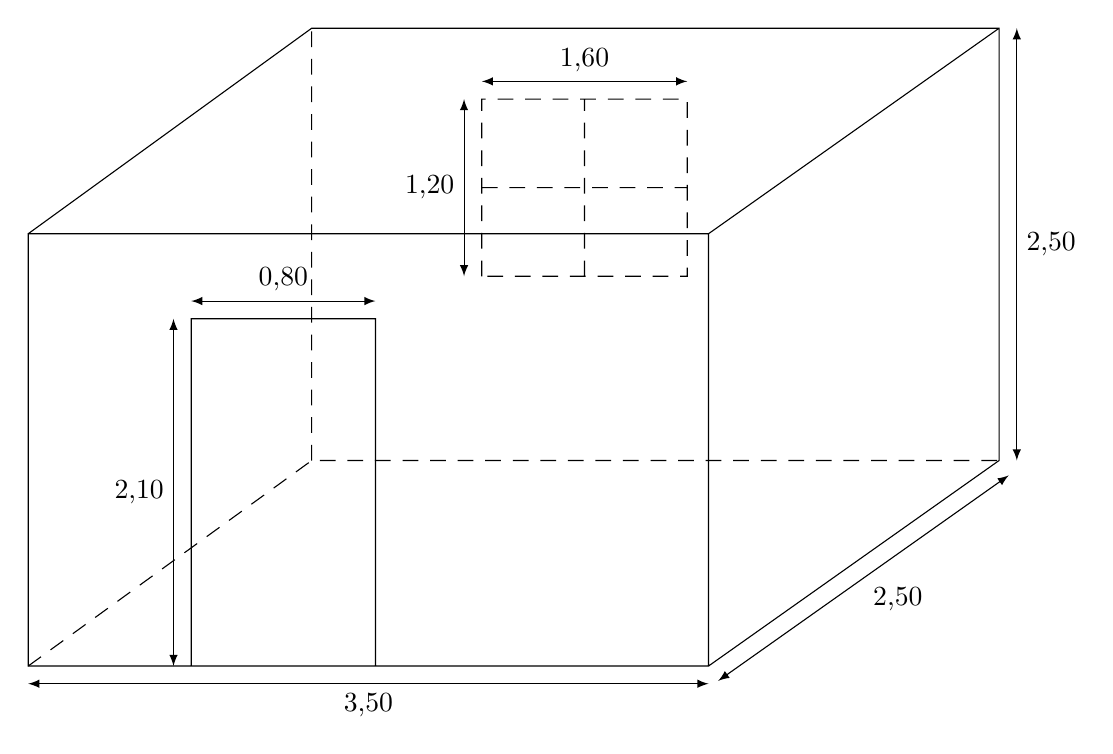
\begin{tikzpicture}[x=0.9cm,y=0.9cm,> = latex]
		\draw  (0,0) rectangle (9.6,6.1)
			   (2.3,0) rectangle (4.9,4.9)	
			   (0,6.1)--(4,9)--(13.7,9)--(13.7,2.9)--(9.6,0)
			   (9.6,6.1)--(13.7,9);
		\draw[dash pattern=on 2mm off 1.5mm] 
				(0,0)--(4,2.9)--(13.7,2.9)
				(4,2.9)--(4,9)
				(6.4,5.5) rectangle (9.3,8)
				(7.85,5.5)--(7.85,8)
				(6.4,6.75)--(9.3,6.75);
		\draw[<->, shift={(0,-0.25)}] (0,0)--(9.6,0)
		node[below,pos=0.5]{3,50};
		\draw[<->, shift={(-57:0.25)}] (9.6,0)--(13.7,2.9)
		node[below right,pos=0.5]{2,50};
		\draw[<->, shift={(0.25,0)}] (13.7,2.9)--(13.7,9)
		node[right,pos=0.5]{2,50};
		\draw[<->, shift={(-0.25,0)}] (2.3,0)--(2.3,4.9)
		node[left,pos=0.5]{2,10};
		\draw[<->, shift={(0,0.25)}] (2.3,4.9)--(4.9,4.9)
		node[above,pos=0.5]{0,80};
		\draw[<->, shift={(-0.25,0)}] (6.4,5.5)--(6.4,8)
		node[left,pos=0.5]{1,20};
		\draw[<->, shift={(0,0.25)}] (6.4,8)--(9.3,8)
		node[above,pos=0.5]{1,60};
	\end{tikzpicture}
\end{center}
	
	On dispose des informations suivantes :
	
	\fbox{\rule[-2.1cm]{0mm}{4.4cm}\begin{minipage}{0.53\linewidth}
			Prix du papier peint :
			
			\begin{itemize}[label=\textbullet,leftmargin=*]
				\item le papier peint est vendu au rouleau entier ;
				
				\item un rouleau coûte 16,95 \euro{};
				\item un rouleau permet de recouvrir 5,3 m$^2$.
			\end{itemize}
			\emph{Conseil du vendeur :} 
			
			prévoir 1 rouleau de papier peint en plus afin de compenser les pertes liées aux découpes.
	\end{minipage}}
	\hfill
	\fbox{\rule[-2.1cm]{0mm}{4.4cm}\begin{minipage}{0.42\linewidth}
		Prix de la colle :
		\begin{itemize}[label=\textbullet,leftmargin=*]
			\item la colle est vendue au pot entier ;
			\item un pot a une masse de 0,2 kg;
			\item un pot coûte 5,70 \euro{}.
		\end{itemize}
				\emph{Conseil du vendeur :}
		
		compter 1 pot de colle pour 4 rouleaux de papier peint.		
	\end{minipage}}

	\begin{enumerate}
		\item Montrer que la surface à recouvrir de papier peint est de 26,4 m$^2$.
		
		\item Calculer le prix, en euro, d’un mètre carré de papier peint.
		Arrondir au centime d'euro.
		
		\item Si on suit les conseils du vendeur, combien coûtera la rénovation de la salle de bain ?
		
		\item Le jour de l'achat, une remise de 8 \% est accordée.
		
		Quel est le prix à payer après remise ? Arrondir au centime d'euro.
	\end{enumerate}

\medskip
\paragraph{Exercice 2}\hfill  \textbf{4 points}

\medskip
\noindent On considère le pavé droit représenté ci-contre tel que :
$AF=3$cm ; $AD=4$cm et $AB=5$cm.

\medskip
\noindent \begin{minipage}{12cm}
\begin{enumerate}
\item \begin{enumerate}
\item Dessiner $ABCD$ en vraie grandeur.
\item Placer le point $K$ milieu de $[BC]$.
\item Calculer la valeur exacte de $AK$.
\end{enumerate}

\medskip
\item Ce pavé est coupé par le plan qui passe par $A$ et $K$ et qui est parallèle à
(BG).
\begin{enumerate}
\item Quelle est la nature de la section ? Justifie soigneusement.
\item Indiquer ses dimensions exactes
\item Représenter cette section en vraie grandeur dans son plan
\end{enumerate}
\end{enumerate}
\end{minipage} 
\hspace{2mm}
\begin{minipage}{4cm}
\begin{flushright}

\includegraphics[scale=0.5]{../40.Image/08. Exo-Espace - sections de solides 7.png}
\end{flushright}
\end{minipage}		

\medskip
\paragraph{Exercice 3}\hfill  \textbf{6 points}

\medskip
Pour chacun des six énoncés suivants, écrire sur la copie le numéro de la question et la réponse choisie. 

Il y a une seule réponse correcte par énoncé. 

\emph{On rappelle que pour valoir des points, les réponses doivent être justifiées.}

\begin{center}
\renewcommand{\arraystretch}{1.5}
\begin{tabularx}{\linewidth}{|c|m{6.5cm}|*{3}{>{\centering \arraybackslash}X|}}\hline
&&\textbf{Réponse A}&\textbf{Réponse B}&\textbf{Réponse C}\\ \hline

1&La forme développée de $(4x+2)(6-2x)$ est : & $8x^2+28x+12$ & $-8x^2+20x+12$ & $-8x^2-28x+12$\\ \hline

2&$6x+8$ est la forme développée de : & $3+(2x+4)$ & $x^2 +8 -x(x-6)$ & $10x-(4x+8)$ \\ \hline
3&Dans la cellule A2 du tableur ci-dessous, on a saisi la formule :

\begin{center}
$= - 5*\text{A}1 * \text{A}1 + 2 * \text{A}1  - 14$
\end{center}

puis on l'a étirée vers la droite.

 Quel nombre obtient-on dans la cellule B2 ?

\begin{center}
 \begin{tableur}{3}
\hline
&\cellcolor{white}{$-4$} & \cellcolor{white}{$-3$}& \cellcolor{white}{}\\\hline
&\cellcolor{white}{$- 102$} & \cellcolor{white}{}& \cellcolor{white}{}\\\hline
\end{tableur}
 \end{center} \arrayrulecolor{black}&$- 65$&205&25\\ \hline
4& La forme développée de $(3x+6)^2$ est : & $3x^2+36$ & $9x^2+36$ & $9x^2+36x+36$\\ \hline
5& $5x+8-4(2x-8)$ est égal à : & $13x+16$ & $9x-16$ & $-3x+16$\\ \hline
6& Quel est le volume d'un cone de rayon $3$cm et de hauteur $10$cm ? & $60\pi$ cm$^3$ &  $20\pi$ cm$^3$ & $30\pi$ cm$^3$\\ \hline
\end{tabularx}
\end{center}
\end{document}